\documentclass[11pt]{article}

\usepackage[a4paper,margin=1in]{geometry}
\usepackage{microtype}
\usepackage{amsmath,amssymb,amsfonts}
\usepackage{hyperref}
\usepackage{float}
\usepackage{placeins}
\usepackage{amsmath}
\usepackage{booktabs} 
\usepackage{array,booktabs,tabularx}
\usepackage{tikz}
\usetikzlibrary{arrows.meta,calc,angles,quotes}

\newcolumntype{L}{>{\raggedright\arraybackslash}X}
\newcommand{\sech}{\operatorname{sech}}


\numberwithin{equation}{section}

\title{Unimetry: A Phase-Space Reformulation of Special Relativity}
\author{Timur Abizgeldin\\ \small Independent researcher, Austria\\ \small \texttt{timurabizgeldin@gmail.com}}
\date{\today}


% --- Unimetry macros ---
\usepackage{tikz}
\usetikzlibrary{arrows.meta,positioning,calc}
\providecommand{\bi}{\mathbf{i}}
\providecommand{\bj}{\mathbf{j}}
\providecommand{\bk}{\mathbf{k}}
\providecommand{\uhat}{\hat{\mathbf u}}
\providecommand{\rotor}[2]{\cos\frac{#2}{2} + #1\,\sin\frac{#2}{2}}

\begin{document}
\maketitle

\begin{abstract}We propose a compact reformulation of special relativity in which spacetime units (time and length) are treated as phase velocities - directional derivatives of a single underlying parameter, the phase $\vec{\chi}\in\mathbb{H}$. The observable Minkowski interval emerges as a conserved quantity under a change of parameter from the phase coordinate $\chi$ to the observer's proper time $\tau$. In this formalism, we show that familiar relativistic effects - time dilation, Lorentz factor, Doppler shift, and relativistic velocity composition - arise as elementary projections and rotations in a Euclidean phase plane. Hyperbolic features of Lorentz kinematics reappear after a reparameterization of time, yielding the standard relations without altering empirical content. We provide closed-form derivations of the longitudinal/transverse Doppler factors, identify a simple lemma equating the total phase speed to the conserved Minkowski norm, and outline connections to gauge phases, rapidity, and a cosmological time gauge. Composition of non-collinear boosts (D-rotations strictly in $\mathbb{H}$) yields a Wigner rotation; in the continuous limit this gives Thomas precession; both arise here as purely kinematical consequences of the quaternionic phase formalism (see §4.7).\end{abstract}

\paragraph{Keywords:} special relativity; phase; rapidity; Doppler shift; Lorentz factor; Wigner rotation; Thomas precession; phase parameterization.

\paragraph{MSC/PhCS:} 83A05; 83-10; 70A05.

\section{Introduction}


We usually take time and space as primitive. The unimetry formalism introduced here suggests a different viewpoint: time and space are derived projections of a single parameter $\vec{\chi}\in\mathbb{H}$ (``phase'') which is suggested the intrinsic phase parameter of an object. In this picture, relativistic effects such as time dilation and the Doppler shift are geometric consequences of phase-vector rotations, when the quaternion algebra unites spatial rotations and boosts. 

The proposal does not modify physics; it reorganizes familiar relations in a simpler language toward formalism of quantum mechanics demonstrating the physical equivalence between Lorentz transformations and Euclidean rotations under proper time parametrization. We will realize the phase kinematics with quaternionic rotors $d=\cos\tfrac{\psi}{2}+\hat{\mathbf u}\sin\tfrac{\psi}{2}$. Throughout, Greek $\theta$ will denote the \emph{external} rotation angle associated with relative motion, while $\zeta$ denotes an \emph{internal} angle associated with the object's intrinsic state (mass/density heuristic). We emphasize that no modification of Einstein's dynamics is proposed; all results are kinematical identities obtained by a change of parameter.

\paragraph{Notation.} Tildes, dots and primes indicate derivatives with respect to the phase parameter, proper time, and spatial arclength:
\[
\tilde{X}:=\frac{dX}{d\chi},\qquad \dot{X}:=\frac{dX}{d\tau},\qquad X':=\frac{dX}{dl}.
\]

\begin{table}[t]
\centering
\caption{Notation used in the paper.}
\label{tab:notation-phase}
\setlength{\tabcolsep}{6pt}
\renewcommand{\arraystretch}{1.1}
\begin{tabularx}{\linewidth}{@{} l L @{}}
\toprule
\textbf{Symbol} & \textbf{Meaning} \\
\midrule
$\tilde{X}$ & Normalized / phase–plane quantity (dimensionless), or a projection as defined at first occurrence. \\
$\dot{X}$    & $dX/dt$ (lab time) by default; derivatives with respect to proper time and phase are written $dX/d\tau$ and $dX/d\vartheta$. \\
$X'$         & Value in a primed inertial frame or after one composition/transform; $X''$ after two compositions. \\
\bottomrule
\end{tabularx}
\end{table}

We use $\mathtt{c}$ for the speed of light; $\beta:=v/\mathtt{c}$, $\gamma:=1/\sqrt{1-\beta^2}$, rapidity $\tanh\eta=\beta$. The subscript $l$ in $dx_l$ denotes spatial components, with $l=1,2,3$ a Cartesian index.

% === BEGIN PATCH (operational phase + mapping + GR) ===

% === New Section: Phase definition and operational meaning ===
\section{\texorpdfstring{Phase: operational definition and physical meaning}{Phase: operational definition}}
% --- patch: angle motivation ---
We will systematically replace hyperbolic functions and nested square roots by the circular trigonometry of a single \emph{phase angle} $\vartheta$, interpreting $\cos\vartheta$ as the temporal projection and $\sin\vartheta$ as the spatial one. This keeps all kinematic identities while avoiding hyperbolic parametrization.  

We define the \emph{kinematic angle} $\vartheta\in[0,\tfrac{\pi}{2})$ of a system with respect to a fixed observer as an \textbf{operationally measurable split} of a constant ``flow budget'' $c$ between temporal and spatial projections:
\begin{equation}
\boxed{\quad \cos\vartheta \equiv \frac{d\tau}{dt}, \qquad \sin\vartheta \equiv \frac{\|\mathbf v\|}{c}=\beta, \quad \mathbf u=\frac{\mathbf v}{\|\mathbf v\|}\quad}
\label{eq:operational-phase}
\end{equation}
where $t$ is the observer's time, $\tau$ is the proper time, and $\mathbf v$ is the 3-velocity. The identity $\cos^2\vartheta+\sin^2\vartheta=1$ then restates the empirical invariance of the Minkowski interval.

\paragraph{Phase state and quaternionic slice.}
An (inertial) phase state is the pair $(\vartheta,\mathbf u)$, with $\mathbf u\in S^2$. We associate to it the unit quaternion
\begin{equation}
q(\vartheta,\mathbf u)=\cos\vartheta + \mathbf I_{\mathbf u}\,\sin\vartheta, \qquad 
\mathbf I_{\mathbf u}:=u_x\,\mathbf i+u_y\,\mathbf j+u_z\,\mathbf k, \ \ \|\mathbf u\|=1,
\end{equation}
that is, a complex slice $\mathbb C_{\mathbf u}:=\mathrm{Span}\{1,\mathbf I_{\mathbf u}\}\subset\mathbb H$ aligned with $\mathbf u$. This is the minimal structure that linearly encodes collinear compositions and naturally induces the Wigner--Thomas rotation for non-collinear boosts via quaternion multiplication.



% === New Section: Mapping to standard SR variables ===
\section{\texorpdfstring{Mapping to standard SR variables}{Mapping to SR}}
The phase angle $\vartheta$ is \emph{not} the rapidity $\eta$; they are related by a Gudermann-type~\cite{Gudermann1830} bridge
\begin{equation}
\boxed{\ \ \beta=\tanh\eta=\sin\vartheta,\qquad \gamma=\cosh\eta=\sec\vartheta,\qquad 
\tan\frac{\vartheta}{2}=\tanh\frac{\eta}{2}\ \ }.
\label{eq:gudermann}
\end{equation}
Consequently, all standard kinematic relations follow from circular trigonometry in $\vartheta$:
\begin{equation}
\gamma=\frac{1}{\sqrt{1-\beta^2}}=\sec\vartheta,\qquad 
k_{\parallel}=e^{\pm\eta}=\frac{1+\tan(\vartheta/2)}{1-\tan(\vartheta/2)}.
\end{equation}
All collinear compositions reduce to angle addition inside the slice $\mathbb{C}_{\mathbf u}$.

\paragraph{Collinear composition.}
For $\mathbf u$ fixed,
\begin{equation}
q(\vartheta_2,\mathbf u)\,q(\vartheta_1,\mathbf u)=q(\vartheta_1\oplus\vartheta_2,\mathbf u),\qquad 
\cos(\vartheta_1\oplus\vartheta_2)=\cos\vartheta_1\cos\vartheta_2-\sin\vartheta_1\sin\vartheta_2,
\end{equation}
which implies Einstein's velocity addition
\begin{equation}
\beta_{12}=\sin(\vartheta_1\oplus\vartheta_2)=\frac{\beta_1+\beta_2}{1+\beta_1\beta_2}.
\end{equation}



\paragraph{Non-collinear composition and Wigner--Thomas rotation.}
For $\mathbf u_1\neq\mathbf u_2$ one has the factorization
\begin{equation}
q(\vartheta_2,\mathbf u_2)\,q(\vartheta_1,\mathbf u_1)=R_W\;q(\vartheta_{12},\mathbf u_{12}),
\end{equation}
where $R_W\in\mathrm{SO}(3)$ is the Wigner--Thomas rotation (a genuine 3D rotation), while $q(\vartheta_{12},\mathbf u_{12})$ is the effective boost in the slice $\mathbb C_{\mathbf u_{12}}$. The rotation angle and axis can be extracted from the vector part of the quaternion product; a closed expression equivalent to the standard formulas is provided in Appendix~\ref{app:1}.



% === New Section: SR ↔ Phase correspondences (table) ===
\section{\texorpdfstring{SR–phase correspondences}{SR–phase correspondences}}
Below is a minimal dictionary of correspondences between the hyperbolic SR picture and the circular phase picture.
\begin{table}[H]
\centering
\begin{tabular}{@{}lll@{}}
\toprule
Quantity & Standard SR (hyperbolic) & Phase picture (circular) \\
\midrule
Rapidity & $\eta=\operatorname{artanh}\beta$ & $\tanh\eta=\sin\vartheta$ \\
Lorentz factor & $\gamma=\cosh\eta$ & $\gamma=\sec\vartheta$ \\
Speed & $\beta=\tanh\eta$ & $\beta=\sin\vartheta$ \\
Doppler (longitudinal) & $k=e^{\pm\eta}$ & $k=\dfrac{1+\tan(\vartheta/2)}{1-\tan(\vartheta/2)}$ \\
Temporal projection & $\sech\eta$ & $\cos\vartheta$ \\
\bottomrule
\end{tabular}
\caption{One-to-one correspondences between hyperbolic (rapidity) and circular (phase) parametrizations.}
\label{tab:correspondence}
\end{table}

\begin{figure}[!ht]
\centering
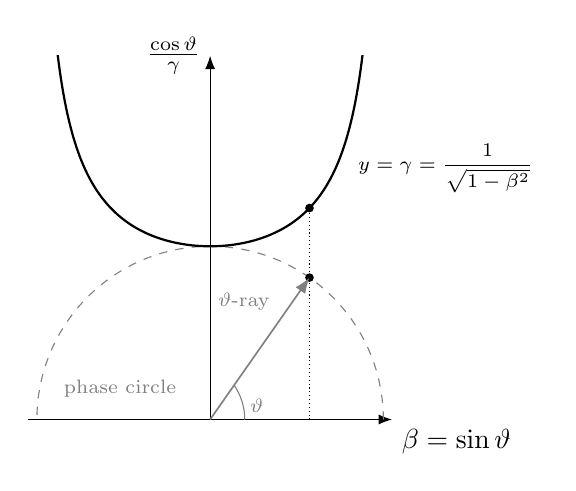
\begin{tikzpicture}[scale=2.2, >=Latex]
  % общие параметры
  \def\ymax{2.1}
  \def\th{35} % пример угла
  \pgfmathsetmacro{\bet}{sin(\th)}   % β = sin θ
  \pgfmathsetmacro{\co}{cos(\th)}    % cos θ
  \pgfmathsetmacro{\ga}{1/\co}       % γ = sec θ

  % оси (вне clip, чтобы надписи не резались)
  \draw[->] (-1.05,0) -- (1.05,0) node[below right] {$\beta=\sin\vartheta$};
  \draw[->] (0,0) -- (0,\ymax) node[left] {$\frac{\cos\vartheta}{ \gamma}$};

  \begin{scope}
    \clip (-1.05,0) rectangle (1.95,\ymax);

    \draw[gray,dashed] (0,0) circle (1);

    \draw[line width=0.8pt] plot[domain=-0.90:0.90, samples=240] (\x, {1/sqrt(1-\x*\x)});

    \draw[densely dotted] (\bet,0) -- (\bet,\ga);
    \fill (\bet,\co) circle (0.025);
    \fill (\bet,\ga) circle (0.025);
  \end{scope}

  \draw[gray,->,line width=0.6pt] (0,0) -- (\bet,\co) node[pos=0.7, above left] {\scriptsize $\vartheta$-ray};
  \draw[gray] (0.20,0) arc[start angle=0, end angle=\th, radius=\th/100];
  \node[gray] at (0.27,0.08) {\scriptsize $\vartheta$};

  \node[gray] at (-0.52,0.18) {\scriptsize phase circle};
  \node at (1.36,1.45) {\scriptsize $y=\gamma=\dfrac{1}{\sqrt{1-\beta^{2}}}$};
\end{tikzpicture}
\caption{Phase circle vs. Lorentz hyperbola at common $\beta=\sin\vartheta$. Vertical mapping at fixed $\beta$ illustrates the Gudermann bridge: $\gamma=\sec\vartheta=\cosh\eta$.}
\label{fig:circle-hyperbola-gd}
\end{figure}
\FloatBarrier

\section{Time and space as phase derivatives}

\paragraph{Why a complex slice of a quaternion?}
For local kinematics any unit direction $\uhat$ singles out the two--dimensional subalgebra
$\mathrm{Span}\{1,\uhat\}\cong\mathbb{C}\subset\mathbb{H}$. Working in this complex
\emph{slice} preserves all boost/rotation algebra along $\uhat$, but keeps formulas
elementary. When the direction changes, one updates the slice; the full quaternionic
structure is retained.

Let $\vec{\chi}\in\mathbb{C}$ be a variable whose change generates observable time-space effects. We treat the time and space units as directional derivatives (phase velocities) along the real and imaginary directions of a complex basis $(\hat{h},\mathbf{l})$:
\begin{equation}
\hat{h}\,dx_0=\frac{\partial\vec{\chi}}{\partial\chi_h}\frac{d\chi_h}{d\chi}\,d\chi
=\tilde{H}\,d\chi,\qquad
\mathbf{l}\,dx_l=\frac{\partial\vec{\chi}}{\partial\chi_l}\frac{d\chi_l}{d\chi}\,d\chi
=\tilde{L}\,d\chi,\quad l=1,2,3.
\label{eq:11}
\end{equation}
Introduce the phase speed of the SR interval $ds=\tilde{S}\,d\chi$. The interval conservation takes the form
\begin{equation}
\tilde{S}^2=\frac{ds^2}{d\chi^2}
=\frac{g_{ij}\,dx^i dx^j}{d\chi^2}
=\left( \frac{\mathtt{c}^2 dt^2}{d\chi^2} \right) - \left[ \frac{\mathbf{dx}^2}{d\chi^2} \right]
=\left( \tilde{H}^2 \right) - \left[ \tilde{L}^2 \right],
\label{eq:12}
\end{equation}
equivalently
\begin{equation}
\tilde{H}^2=\tilde{S}^2+\tilde{L}^2.
\label{eq:13}
\end{equation}
Writing 
\begin{equation}
\tilde{S}=\tilde{H}\cos\theta,\qquad \tilde{L}=\tilde{H}\sin\theta,
\label{eq:14}
\end{equation}
where $\theta$ is the angle of the phase speed relative to the real axis. Algebraically, \eqref{eq:13} is a Euclidean decomposition of a single speed into orthogonal projections; physically, we will see that under reparameterization the \emph{projection} $\tilde{S}$, not the Euclidean norm $\tilde{H}$, is the conserved Minkowski quantity.

% --- patch: Flow and phase 1-form ---
\paragraph{Flow and phase 1-form.}
Let $\Phi:\mathcal E\to\mathbb R$ be a scalar \emph{phase potential} on a (possibly infinite-dimensional) Euclidean/Hilbert proto-space $(\mathcal E,\langle\cdot,\cdot\rangle)$. 
Define the phase 1-form $\alpha:=d\Phi$ and the associated \emph{flow vector} $\boldsymbol\chi:=\nabla\Phi$, where the gradient is taken with respect to $\langle\cdot,\cdot\rangle$.

Fix an observer's orthonormal spatial triad $\{\mathbf e_1,\mathbf e_2,\mathbf e_3\}\subset\mathcal E$ and let $S=\mathrm{span}\{\mathbf e_1,\mathbf e_2,\mathbf e_3\}$ with orthogonal projectors $P_S$ and $P_{S^\perp}$. 
Decompose
\[
\boldsymbol\chi=\boldsymbol\chi_S+\boldsymbol\chi_\perp,\qquad
\boldsymbol\chi_S:=P_S\boldsymbol\chi,\quad 
\boldsymbol\chi_\perp:=P_{S^\perp}\boldsymbol\chi.
\]
Define observable spatial components and the orthogonal magnitude
\[
\ell_i:=\langle\boldsymbol\chi,\mathbf e_i\rangle,\qquad 
\mathbf l:=\sum_{i=1}^3 \ell_i\,\mathbf e_i,\qquad 
t:=\|\boldsymbol\chi_\perp\|=\sqrt{\|\boldsymbol\chi\|^2-\|\boldsymbol\chi_S\|^2},
\]
and, for orientation when $t>0$, the unit direction $\mathbf e_t:=\boldsymbol\chi_\perp/\|\boldsymbol\chi_\perp\|$.
Then the phase angle $\vartheta$ and the direction $\mathbf u$ used throughout this paper are recovered as
\[
\cos\vartheta=\frac{t}{\|\boldsymbol\chi\|},\qquad 
\sin\vartheta=\frac{\|\mathbf l\|}{\|\boldsymbol\chi\|},\qquad 
\mathbf u=\frac{\mathbf l}{\|\mathbf l\|}\quad(\|\mathbf l\|>0).
\]
This complements the operational definition \eqref{eq:operational-phase} and ties the phase picture to a differential-form language.


\section{Phase space}
Let the phase vector space be $\mathbb{H}$ with orthonormal basis $(\hat{h},\mathbf{l})$. For a phase vector $\vec{\chi}=R\,e^{\theta\mathbf{l}}$ with $\theta\in[-\pi,\pi]$,
\begin{equation}
\tilde{H}=R,\qquad \tilde{S}=R\cos\theta,\qquad \tilde{L}=R\,\mathbf{l}\sin\theta.
\label{eq:21}
\end{equation}
Choosing coordinates where the projectors onto $(\hat{h},\mathbf{l})$ are unit, \eqref{eq:11} simplifies to
\begin{equation}
\hat{h}\,dx_0=\frac{d\chi_h}{d\chi}\,d\chi=\tilde{H}\,d\chi,\qquad
\mathbf{l}\,dx_l=\frac{d\chi_l}{d\chi}\,d\chi=\tilde{L}\,d\chi.
\label{eq:22}
\end{equation}
The map from phase to observables is an integral transform:
\begin{equation}
x^i(\chi)=x^i(\chi_0)+\int_{\chi_0}^{\chi}\tilde{X}^i(u)\,du,\qquad i=0,1,2,3,
\label{eq:23}
\end{equation}
where $\tilde{X}^i$ are projections of $d\vec{\chi}/d\chi$ onto $(\hat{h},\mathbf{l})$ and $x^i(\chi_0)$ fix initial conditions.

\section{Objects}
\noindent\textit{Roadmap.} The next formulas fix notation and the geometric carriers we use throughout. 
In particular, the phase state $(\vartheta,\mathbf u)$ selects a complex slice 
$\mathbb C_{\mathbf u}\subset\mathbb H$; collinear compositions become ordinary circular sums on this slice, 
while non-collinear compositions generate a genuine 3D rotation (Wigner–Thomas) via quaternion multiplication.
This explains why we keep both $\vartheta$ and $\mathbf u$ as primary objects.

A fundamental particle is an elementary object with nonzero phase $\vec{\chi}\neq0$. Composite objects are phase configurations; to represent them in phase space one may require additional dimensions, except for the photon, whose phase is always aligned with the imaginary axis:
\begin{equation}
\mathbf{p}=\frac{d\vec{\chi}}{d\chi_l}=p\,\mathbf{l}\in\Im.
\label{eq:31}
\end{equation}
Non-photonic phenomena are associated with nonzero real projection and nonzero mass. A complex object can be identified with an event or worldline; the photon corresponds to a null-interval point encoding information about the event.

Any object's phase can be rotated to the \emph{zero} (purely real) direction,
\begin{equation}
\vec{\chi}_0=R\in\Re.
\label{eq:32}
\end{equation}
An object $A$ moving with speed $v$ relative to a rest observer has
\begin{equation}
\vec{\chi}_A=R\,e^{\theta_A\mathbf{l}},\qquad
\sin\theta_A=\frac{v}{\mathtt{c}}\equiv\beta.
\label{eq:33}
\end{equation}

\noindent\textit{From unit norm to the interval.}
We will repeatedly use that $cd\tau= c\,dt\,\cos\vartheta$ and $d\mathbf x=c\,dt\,\sin\vartheta\,\mathbf u$.
Thus the identity $\cos^{2}\vartheta+\sin^{2}\vartheta=1$ is exactly the Minkowski metric statement 
$(cd\tau)^{2}=(cdt)^{2}-d\mathbf x^{2}$; from now on, square-root expressions are traded for circular 
trigonometry in $\vartheta$.


\subsection{Space as a symmetric phase pair}
From \eqref{eq:14}, a naive zero-angle limit would remove the imaginary projection, contradicting observability. We enforce a nonvanishing spatial projection by pairing opposite-phase tilts:
\begin{equation}
\vec{\chi}^{\pm}=R\,e^{\pm\zeta\,\mathbf{l}},\qquad
\vec{\chi}_l:=\frac{\vec{\chi}^+-\vec{\chi}^-}{2}=R\,\mathbf{l}\sin\zeta,
\label{eq:311}
\end{equation}
where $\zeta$ is an \emph{internal angle} (intrinsic to the object; heuristically linked to mass/density). The local decomposition is
\begin{equation}
\vec{\chi}_0=\vec{\chi}_\tau+\vec{\chi}_l
=R\cos\zeta+R\,\mathbf{l}\sin\zeta,
\label{eq:312}
\end{equation}
with unit components (normalized by $R$): the real component is $\cos\zeta$ and the imaginary component is $\sin\zeta$.

\subsection{Absolute, local, and observed time}
Define \emph{absolute} time $t=t(\tilde{H})$ at the zero phase direction; it is the fastest clock and useful for normalization between different phase speeds. Along the local real direction,
\begin{equation}
dx_0=\frac{d}{d\chi}\Re(\vec{\chi})\,d\chi
=\frac{\vec{\chi}^+ + \vec{\chi}^-}{2}\,d\chi
=\cos\zeta\,d\chi
=:d\tau.
\label{eq:321}
\end{equation}
Here $d\chi_0:=\cos\zeta\,d\chi$ is the projection of $d\chi$ onto the local real axis; in Sec.~\ref{sec:norm} we calibrate $d\tau=(1/\nu_0)\,d\chi_0$. The observed proper time of $A$ relative to the rest observer is
\begin{equation}
\tilde{H}_A=\Re\!\left(\frac{d\vec{\chi}_A}{d\vec{\chi}_0}\right)
=\cos\theta_A
=\sqrt{1-\sin^2\theta_A}
=\sqrt{1-\frac{v^2}{\mathtt{c}^2}}
=\frac{1}{\gamma}.
\label{eq:322}
\end{equation}

\subsection{Normalization}\label{sec:norm}
\noindent\textit{Calibration.}
We fix the calibration by the observer’s clock and speed budget: 
$\cos\vartheta \equiv d\tau/dt$ and $\sin\vartheta \equiv \beta$.
This choice does not restrict generality: any overall rescaling of the underlying flow is absorbed into the 
definitions of $t$ and $c$, leaving all dimensionless observables unchanged.

Let local time be parameterized by \emph{phase}; introduce a reference frequency $\nu_0$ and set
\begin{equation}
d\tau=\frac{1}{\nu_0}\,d\chi_0.
\label{eq:331}
\end{equation}
By the chain rule,
\begin{equation}
dx_0=\tilde{H}\,d\chi
=\frac{dx_0}{d\chi_0}\frac{d\chi_0}{d\tau}\,d\tau
=\tilde{H}\,\dot{\chi}\,d\tau
=: \dot{H}\,d\tau,
\label{eq:332}
\end{equation}
where $\nu:=d\chi/d\tau$, $\dot{\chi}:=\nu/\nu_0$, and $\dot{H}:=\tilde{H}\,\dot{\chi}$. Choosing the calibration $\dot{H}\equiv \mathtt{c}$ gives $dx_0=\mathtt{c}\,d\tau$. Similarly for space,
\begin{equation}
dx_l=\tilde{L}\,d\chi
=\frac{dx_l}{d\chi_0}\frac{d\chi_0}{dl}\,dl
=\tilde{L}\,\chi'\,dl
=:L'\,dl,\qquad \chi':=\frac{d\chi}{dl}.
\label{eq:333}
\end{equation}
From $dx_0=dx_l$ for light one gets
\begin{equation}
\mathtt{c}=\tilde{L}'\,\frac{dl}{d\tau},
\label{eq:334}
\end{equation}
hence with temporal calibration to $\mathtt{c}$ the spatial scale becomes unit: $\tilde{L}'=1$.

\subsection{\texorpdfstring{Light and $\mathtt{c}$ as a calibration constant}{Light and c as a calibration constant}}
From the normalized forms,
\begin{equation}
\frac{\mathtt{c}}{\dot{\chi}}\,d\chi=\frac{1}{\chi'}\,d\chi
\quad\Rightarrow\quad
\mathtt{c}=\frac{\dot{\chi}}{\chi'}=\frac{dl}{d\tau},
\label{eq:341}
\end{equation}
i.e.\ $\mathtt{c}$ is a \emph{calibration constant} tying temporal and spatial measures, independent of local phase variation. Equation \eqref{eq:341} also reads
\begin{equation}
\mathtt{c}=\left(\frac{d\chi}{d\tau}\right)\!\left[\frac{dl}{d\chi}\right]\sim (\nu)\,[\lambda],
\label{eq:343}
\end{equation}
matching frequency and wavelength of a photon, with $\chi$ as its phase. For a lightlike trajectory,
\begin{equation}
ds^2=\mathtt{c}^2\!\left(\frac{d\chi^2}{\dot{\chi}^2}-\frac{d\chi^2}{\dot{\chi}^2}\right)=0.
\label{eq:344}
\end{equation}
At unit frequency, $\tau=\chi$: the photon's ``proper time'' is its phase, and the length of its phase-speed vector equals its wavelength, $\tilde{H}_p=\lambda$. Finally, the kinematic slope in phase coordinates is
\begin{equation}
\frac{dx_l}{dx_0}
=\frac{\tilde{L}\,d\chi}{\tilde{H}\,d\chi}
=\sin\theta
=\frac{v}{\mathtt{c}}
\equiv \beta,
\label{eq:345}
\end{equation}
so $\theta=\pi/2$ implies $v=\mathtt{c}$.

\subsection{Lorentz factor via reparameterization}
A change of direction of the phase speed transforms
\begin{equation}
\tilde{H}^2=\tilde{S}^2+\tilde{L}^2 \;\longmapsto\;
\dot{H}^2=\dot{S}^2+\dot{L}^2.
\label{eq:351}
\end{equation}
\textbf{Lemma (parameter-change identity).} The transition $\tilde{H}\to\dot{S}$ is the manifestation of evolving phase speed under the parameter change $\chi\mapsto \tau(\chi)$, with local Jacobian
\begin{equation}
\frac{d\tau}{d\chi}=\cos\zeta(\chi)\cos\theta(\chi)
\quad\Rightarrow\quad
\mathcal{J}(\zeta,\theta):=\frac{d\chi}{d\tau}=\frac{1}{\cos\zeta\,\cos\theta}.
\label{eq:353}
\end{equation}
Then
\begin{equation}
\dot{H}=\tilde{H}\,\mathcal{J},\qquad \dot{L}=\tilde{L}\,\mathcal{J}.
\label{eq:354}
\end{equation}
In differential form,
\begin{equation}
d\ln\dot{H}=d\ln\mathcal{J}=\tan\zeta\,d\zeta+\tan\theta\,d\theta.
\label{eq:355}
\end{equation}
For a \emph{pure boost} ($d\zeta=0$) one has $d\dot{H}=\dot{H}\tan\theta\,d\theta$. Absorbing a constant $\cos\zeta$ into the calibration (set $\zeta=0$ henceforth), we obtain
\begin{equation}
\tilde{H}^2=\dot{H}^2-\dot{L}^2=\sec^2\theta\,(\tilde{H}^2-\tilde{L}^2)=\gamma^2(\tilde{H}^2-\tilde{L}^2).
\label{eq:356}
\end{equation}
\textbf{Corollary.} In phase space the Euclidean norm $\tilde{H}$ is conserved; in observed time the Minkowski norm $\dot{S}$ is conserved; they are identical as quantities:
\begin{equation}
\boxed{\ \tilde{H}=\dot{S}\ }.
\label{eq:357}
\end{equation}

\subsection{Rapidity and the phase angle}
By definition,
\begin{equation}
\beta=\frac{v}{\mathtt{c}}=\sin\theta,\qquad \tanh\eta=\beta,\qquad
d\eta=\frac{d\beta}{1-\beta^2}.
\label{eq:361}
\end{equation}
With $d\beta=\cos\theta\,d\theta$ and $1-\beta^2=\cos^2\theta$,
\begin{equation}
d\eta=\sec\theta\,d\theta,\qquad
\eta(\theta)=\int\sec\theta\,d\theta
=\ln|\sec\theta+\tan\theta|
=\tfrac12\ln\frac{|1+\sin\theta|}{|1-\sin\theta|}.
\label{eq:364}
\end{equation}
Fixing $\eta(0)=0$,
\begin{equation}
e^{\eta(\theta)}=\sqrt{\frac{1+\sin\theta}{1-\sin\theta}},\qquad
\gamma=\frac{1}{\sqrt{1-\beta^2}}=\sec\theta=\cosh\eta.
\label{eq:365}
\end{equation}

\paragraph{Remark (groups).} Observables satisfy $\beta=\sin\theta=\tanh\eta$ and $\gamma=\sec\theta=\cosh\eta$. Thus Euclidean rotations in the phase circle (\,$U(1)$ with angle $\theta$\,) reproduce the numerical factors of hyperbolic boosts in $SO^+(1,1)$ (rapidity $\eta$) \emph{after} reparameterizing time. We do not claim an isomorphism $U(1)\cong SO(1,1)$; only the equality of observable combinations under the change of parameter.

\subsection{Velocity addition}
\label{sec:vel-addition}

\paragraph{Notation.}
In unimetry, an inertial boost is a \emph{D-rotation}
\begin{equation}
\label{eq:auto:32}
\mathcal{B}(\uhat,\psi):\quad \mathbf q \mapsto d\,\mathbf q\,d,
\qquad
d=\cos\frac{\psi}{2}+\uhat\,\sin\frac{\psi}{2},
\end{equation}
and a spatial rotation is an \emph{R-rotation}
\begin{equation}
\label{eq:auto:33}
\mathcal{R}(\hat{\mathbf n},\varphi):\quad \mathbf q \mapsto r\,\mathbf q\,r^{-1},
\qquad
r=\cos\frac{\varphi}{2}+\hat{\mathbf n}\,\sin\frac{\varphi}{2}.
\end{equation}
Kinematic mapping: $\beta\equiv v/c=\sin\psi$, $\gamma=1/\cos\psi$,
$\displaystyle \tan\frac{\psi}{2}=\frac{\gamma\beta}{\gamma+1}$.
For quaternionic/GA accounts of rotors and Lorentz boosts see \cite{Hamilton1844,HestenesSobczyk1984,DoranLasenby2003}.

\subsubsection{Wigner rotation}
\label{subsec:wigner}

Let $d_1,d_2$ be D-rotors of two successive boosts. The raw action on any unimetry 4-object is
\begin{equation}
\label{eq:auto:34}
\mathbf q' = d_2 d_1\, \mathbf q\, d_1 d_2 \equiv L_{12}\,\mathbf q\,L_{21},\qquad
L_{12}=d_2 d_1,\ \ L_{21}=d_1 d_2.
\end{equation}
Define $d_{12}$ to be the unique D-rotor reproducing the combined spatio--temporal tilt of $L_{12}$:
\begin{equation}
\boxed{\, d_{12}\,\mathbf e_t\, d_{12} \;=\; L_{12}\,\mathbf e_t\, L_{21},\qquad \Re(d_{12})\ge0 \,}
\label{eq:d12-uniqueness}
\end{equation}
(the sign choice removes the trivial two-fold ambiguity). Then the \emph{Wigner rotor} is the residual
R-rotation in the symmetric D--R factorization:
\begin{equation}
\boxed{\, L_{12}=d_{12}\,r_W,\qquad L_{21}=r_W^{-1}\,d_{12} \,}
\label{eq:DR-polar}
\end{equation}
equivalently,
\begin{equation}
\boxed{\, r_W=\bar d_{12}\,L_{12}=L_{21}\,\bar d_{12} \,}.
\label{eq:wigner-rotor-def}
\end{equation}
Hence the observed map after compensating the tilt is $\,\bar d_{12}\,\mathbf q'\,\bar d_{12}=r_W\,\mathbf q\,r_W^{-1}$.

\begin{figure}[!ht]
\centering
\begin{tikzpicture}[>=Latex, node distance=32mm]
  \node (q) {$\mathbf q$};
  \node (d1) [right=of q] {$d_1\,\mathbf q\,d_1$};
  \node (d2) [right=of d1] {$d_2 d_1\,\mathbf q\,d_1 d_2$};
  \node (rw) [below=20mm of d2] {$r_W\,\mathbf q\,r_W^{-1}$};
  \draw[->] (q) -- node[above] {$d_1$} (d1);
  \draw[->] (d1) -- node[above] {$d_2$} (d2);
  \draw[->] (d2) -- node[right] {$\bar d_{12}$ on both sides} (rw);
  \draw[->, dashed, bend left=12] (q) to node[above] {$d_{12}$} (d2);
\end{tikzpicture}
\caption{Two successive D-rotations (boosts) and compensation of the net spatio--temporal angle by the conjugate of $d_{12}$, leaving a pure R-rotation $r_W$.}
\label{fig:tikz-wigner-pullback}
\end{figure}

\subsubsection{Thomas precession}
\label{subsec:thomas}
The continuous limit of Wigner rotation for a time-dependent velocity direction $\uhat(t)$ yields
\begin{equation}
\label{eq:auto:38}
\boldsymbol{\omega}_T=(\gamma-1)\,\bigl(\uhat\times \dot{\uhat}\bigr)
=\frac{\gamma^2}{\gamma+1}\,\frac{\mathbf a\times \mathbf v}{c^2},\qquad
\gamma=\frac{1}{\cos\psi}.
\end{equation}
For uniform circular motion ($|\mathbf v|=\mathrm{const}$) with $\dot{\uhat}=\boldsymbol{\Omega}\times\uhat$ one has
$\lvert\boldsymbol{\omega}_T\rvert=(\gamma-1)\,\Omega$.
\subsection{Doppler shift}
Define the observed frequency as the phase growth rate in the observer's proper time:
\begin{equation}
\nu:=\frac{d\chi}{d\tau}.
\label{eq:381}
\end{equation}
For two successive wavefronts the phase increment is identical, hence
\begin{equation}
\frac{\nu_{\mathrm{obs}}}{\nu_{\mathrm{src}}}
=\frac{d\chi/d\tau_{\mathrm{obs}}}{d\chi/d\tau_{\mathrm{src}}}
=\frac{d\tau_{\mathrm{src}}}{d\tau_{\mathrm{obs}}}.
\label{eq:382}
\end{equation}
Longitudinal case: during $\gamma\,d\tau_{\mathrm{src}}$ in the observer frame the source displaces by $\pm v\,\gamma\,d\tau_{\mathrm{src}}$ (``$+$'' receding, ``$-$'' approaching). Then
\begin{equation}
d\tau_{\mathrm{obs}}=\gamma\,d\tau_{\mathrm{src}}(1\pm\beta),\qquad
\Rightarrow\quad
\boxed{\ \frac{\nu_{\mathrm{obs}}}{\nu_{\mathrm{src}}}=\frac{1}{\gamma(1\pm\beta)}\ }.
\label{eq:384}
\end{equation}
Equivalent forms (with $\beta=\sin\theta$, $\gamma=\sec\theta$ and rapidity $\eta$):
\begin{equation}
\frac{\nu_{\mathrm{obs}}}{\nu_{\mathrm{src}}}
=\sqrt{\frac{1\mp\beta}{1\pm\beta}}
=\sec\theta\,(1\mp\sin\theta)
=e^{\mp\eta}.
\label{eq:385}
\end{equation}
Transverse Doppler ($\varphi=90^\circ$ in the observer's frame):
\begin{equation}
\frac{\nu_{\mathrm{obs}}}{\nu_{\mathrm{src}}}=\frac{1}{\gamma}=\cos\theta.
\label{eq:389}
\end{equation}
General line-of-sight (LOS) angle $\varphi$ in the observer's frame:
\begin{equation}
\boxed{\ \frac{\nu_{\mathrm{obs}}}{\nu_{\mathrm{src}}}=\gamma\,(1-\beta\cos\varphi)\ }.
\label{eq:3810}
\end{equation}
Wavelength ratios are inverse to frequency ratios.

% === Gravity section (moved here) ===
\section{\texorpdfstring{Gravity as a phase rotation: local tetrads and clock angle}{Gravity as a phase rotation}}

On a curved background $(\mathcal M,g)$ we work with orthonormal tetrads $e_a{}^\mu$ such that $g_{\mu\nu}e_a{}^\mu e_b{}^\nu=\eta_{ab}$ and take the observer's time leg to be $e_0{}^\mu$. 
We introduce the \emph{gravitational (clock) angle} $\varphi$ by
\begin{equation}
\cos\varphi\ :=\ e^0{}_\mu\,u^\mu\ =\ \frac{d\tau_{\rm stat}}{dt}\ =\ \sqrt{-g_{00}}\qquad\text{(stationary case)}.
\label{eq:clock-angle}
\end{equation}
Kinematics remains encoded by the phase angle $\vartheta$ in the slice $\mathbb C_{\mathbf u}$, with
$\cos\vartheta=d\tau/d\tau_{\rm stat}$. 
Therefore the proper time factorizes as
\begin{equation}
d\tau\ =\ dt\,\cos\varphi\,\cos\vartheta,\qquad 
d\mathbf x\ =\ c\,dt\,\sin\vartheta\,\mathbf u,
\label{eq:tau-factorization}
\end{equation}
and the total redshift factorizes into kinematic and gravitational parts:
\begin{equation}
1+z_{\rm tot}\ =\ \frac{\cos\vartheta_{\rm em}}{\cos\vartheta_{\rm obs}}\ \times\ 
\frac{\cos\varphi(x_{\rm em})}{\cos\varphi(x_{\rm obs})}.
\label{eq:z-factorization}
\end{equation}
For static emitter/observer ($\vartheta_{\rm em}=\vartheta_{\rm obs}=0$) one recovers the standard gravitational redshift 
$1+z_g=\sqrt{\frac{-g_{00}(x_{\rm obs})}{-g_{00}(x_{\rm em})}}$.
In the weak-field limit $g_{00}\simeq-(1+2\Phi/c^2)$ this gives $z_g\simeq(\Phi_{\rm obs}-\Phi_{\rm em})/c^2$.

\paragraph{Beyond static fields.}
In a $3\!+\!1$ split $ds^2=-N^2 c^2 dt^2 + h_{ij}(dx^i+N^i dt)(dx^j+N^j dt)$ one may identify $\cos\varphi:=N$ in the observer's tetrad, which keeps \eqref{eq:tau-factorization}–\eqref{eq:z-factorization} coordinate-agnostic.
Uniform acceleration (Rindler) accumulates phase according to $d\vartheta=\kappa\,dt$ inside the local slice, consistently reproducing accelerated-frame kinematics when combined with the clock angle $\varphi$.


\section{Discussion: links to known structures}
\paragraph{Gauge phases.} A global shift $\chi\mapsto\chi+\chi_0$ is unobservable. Allowing local reparameterizations $\chi\mapsto\chi+\alpha(x)$ induces a connection when comparing phases at different points. On wavefunctions $\psi\sim e^{i\chi}$ this is the familiar $U(1)$ gauge freedom $\psi\to e^{i\alpha(x)}\psi$ with $D_\mu=\partial_\mu-iA_\mu$ as the \emph{phase-transport connection}.

\paragraph{Mass and the internal angle.} With the decomposition by $\zeta$, mass heuristically correlates with an irreducible real projection: massless objects have $\zeta=\pm\pi/2$ (no proper time; photon subspace), while massive objects have $|\zeta|<\pi/2$ (proper time exists). In the present paper we set $\zeta=0$ in boost kinematics by calibration; a detailed mass-generation mechanism is left for future work.

\paragraph{Cosmological gauge.} A natural global calibration of ``absolute'' time is the comoving frame with vanishing CMB dipole. This fixes a cosmological time $t$ (FLRW) as a gauge, without affecting local Lorentz invariance; Doppler factors are then operationally referenced to that frame.

\section{Conclusion}
In unimetry, time and space are integrals of phase velocities; the Minkowski interval appears as a conserved quantity under parameter change. The core relations of SR---$\gamma$, rapidity, velocity addition, and Doppler factors---follow from elementary phase-plane geometry with a single rotation angle $\theta$, while hyperbolic structure re-emerges upon reparameterizing time. The formalism is empirically equivalent to standard SR but can clarify causality and composition by treating all effects as projections of a single flow.

\paragraph{Outlook.} Future directions include (i) a more explicit group-theoretic embedding, (ii) a rigorous treatment of the internal angle $\zeta$ and its relation to mass, and (iii) exploration of curved metrics as spatially varying Jacobians $\mathcal{J}(x)$ in the phase-to-observable map.

\bibliographystyle{plain}
\begin{thebibliography}{9}
\bibitem{Gudermann1830}  NIST Digital Library of Mathematical Functions, §4.23 ``Gudermannian Function'', \url{https://dlmf.nist.gov/4.23}.

\bibitem{Einstein1905}
A.~Einstein.
\newblock Zur Elektrodynamik bewegter K\"{o}rper.
\newblock {\em Annalen der Physik}, 17:891--921, 1905.
(English translation: On the electrodynamics of moving bodies.)

\bibitem{Rindler}
W.~Rindler.
\newblock {\em Relativity: Special, General, and Cosmological}.
\newblock Oxford University Press, 2nd ed., 2006.

\bibitem{TaylorWheeler}
E.~F. Taylor and J.~A. Wheeler.
\newblock {\em Spacetime Physics}.
\newblock W. H. Freeman, 2nd ed., 1992.

\bibitem{Hamilton1844}
W.~R.~Hamilton,
\newblock \emph{On quaternions; or on a new system of imaginaries in algebra}, Philosophical Magazine \textbf{25}, 10--13 (1844).

\bibitem{HestenesSobczyk1984}
D.~Hestenes and G.~Sobczyk,
\newblock \emph{Clifford Algebra to Geometric Calculus}, Reidel, 1984.

\bibitem{DoranLasenby2003}
C.~Doran and A.~Lasenby,
\newblock \emph{Geometric Algebra for Physicists}, Cambridge University Press, 2003.

\end{thebibliography}




\appendix
\section{Equivalence to the classical Wigner rotation}
\label{app:1}

We sketch an intrinsic quaternionic proof that the unimetry expression for the Wigner rotation
coincides with the standard special-relativistic formula.

\paragraph{Step 1: product of two D-rotors.}
For $d_i=\cos\frac{\psi_i}{2}+\uhat_i\sin\frac{\psi_i}{2}$,
\begin{equation}
\label{eq:auto:45}
d_2 d_1
=(c_2c_1-s_2s_1\cos\theta)
+\Big(c_2s_1\uhat_1+s_2c_1\uhat_2+s_2s_1\,\uhat_2\times\uhat_1\Big),
\end{equation}
with $c_i=\cos(\psi_i/2)$, $s_i=\sin(\psi_i/2)$ and $\cos\theta=\uhat_2\!\cdot\!\uhat_1$.

\paragraph{Step 2: symmetric D--R factorization.}
Define $d_{12}$ by $d_{12}\,\mathbf e_t\, d_{12}=L_{12}\,\mathbf e_t\, L_{21}$ and set
$r_W=\bar d_{12}\,L_{12}=L_{21}\,\bar d_{12}$. Then $r_W$ fixes $\mathbf e_t$ and is a pure spatial
rotor, so $r_W=\cos\frac{\phi}{2}+\hat{\mathbf n}\sin\frac{\phi}{2}$ with
$\hat{\mathbf n}\parallel \uhat_2\times\uhat_1$. Matching scalar and bivector parts gives
\begin{equation}
\tan\frac{\phi}{2}=
\frac{s_1 s_2\,\sin\theta}{\,c_1 c_2+s_1 s_2\,\cos\theta\,}.
\label{eq:uni-phi}
\end{equation}

\paragraph{Step 3: map to rapidities.}
With the substitutions $\sin(\psi/2)\mapsto\sinh(\eta/2)$, $\cos(\psi/2)\mapsto\cosh(\eta/2)$,
$\tan(\psi/2)\mapsto\tanh(\eta/2)$ (where $\tanh\eta=\beta$, $\cosh\eta=\gamma$), \eqref{eq:uni-phi}
becomes the textbook Wigner angle:
\begin{equation}
\label{eq:auto:47}
\tan\frac{\phi}{2}
=\frac{\sinh\frac{\eta_1}{2}\,\sinh\frac{\eta_2}{2}\,\sin\theta}
{\cosh\frac{\eta_1}{2}\,\cosh\frac{\eta_2}{2}+\sinh\frac{\eta_1}{2}\,\sinh\frac{\eta_2}{2}\,\cos\theta},
\end{equation}
with axis along $\uhat_2\times\uhat_1$. This circular--hyperbolic correspondence is classical; cf.\ Gudermann~\cite{Gudermann1830}.



\end{document}
